\documentclass[a4paper,10pt,titlepage]{article}
% PREUMBULUM
\usepackage[utf8]{inputenc}
\usepackage[T1]{fontenc}

\usepackage{a4wide} 
\usepackage{times}

\usepackage[magyar,english]{babel}

% Forráskódoknak:
\usepackage{listings}

% Tartalomjegyzék:
\usepackage{tocbibind}

\usepackage[usenames,dvipsnames]{color}

% Hogy legyen képünk:
\usepackage{graphicx}

%###############################################################################
\newcommand{\szerzo}{Szerző(k)}
\newcommand{\szerzomail}{szerzok@email.org}
\newcommand{\cim}{Cím}
\newcommand{\targy}{}
\newcommand{\kulcsszavak}{}

\usepackage{hyperref}
\hypersetup{
    unicode=true,
    colorlinks=true,
    linkcolor=RoyalBlue,
    citecolor=RoyalBlue,
    filecolor=RoyalBlue,
    urlcolor=RoyalBlue,
    pdftitle={\cim},        % title
    pdfauthor={\szerzo},    % author
    pdfsubject={\targy}, % subject of the document
    pdfcreator={},   % creator of the document
    pdfproducer={LaTeX, TexMaker},    % producer of the document
    pdfkeywords={\kulcsszavak},    % list of keywords
}

\usepackage{url}

% Táblázatoknak:
\usepackage{colortbl}

% Ha kell matek:
\usepackage{amssymb,amsmath}

\usepackage{verbatim} % Hogy lehessen blokkkommentezni

% Egymás melleti képekhez:
\usepackage{subfig}

\setlength{\parindent}{12pt} % magyar nyelvű dokumentumokban jellemző
\setlength{\parskip}{0pt}    % magyar nyelvű dokumentumokban jellemző

\usepackage{setspace}  % Ettol a tablazatok, abrak, labjegyzetek maradnak 1-es sorkozzel!

%###########################################
% Saját eszközök:
%
\definecolor{todobgszin}{rgb}{0.64,0.78,0.22}
\definecolor{todofrszin}{rgb}{0.00,0.50,0.00}

\newcommand{\angolul}[1]{\foreignlanguage{english}{#1}}

\newcommand{\todo}[1]{
    \vfill
    \begingroup % Csinálunk egy csoportot, hogy az identálás csak erre vonatkozzon
        \setlength{\parindent}{0cm} % Beállítjuk, hogy teljes szélességű legyen a dobozunk a bekezdéstől függetlenül
        \fcolorbox{todofrszin}{todobgszin}{
            \parbox{\textwidth}{
                \vskip10pt
                \leftskip10pt
                \rightskip10pt
            
                \emph{TODO: #1}
  
                \vskip10pt
            }
        }
    \endgroup
    \vfill
}

\newenvironment{sajat_itemize}
{
	\begin{itemize}
	\setlength{\itemsep}{0pt}
}
{
	\end{itemize}
}

\begin{document}
% Dokumentumtörzs

\selectlanguage{magyar}

% Címoldal:
\begin{titlepage}

\title{\cim}
\author{\szerzo \\ < \szerzomail >}
\date{\today}

\end{titlepage}
\maketitle

% Nem akarom, hogy megjelenjen a tartalomjegyzékben a Tartalomjegyzék:
\section*{Tartalomjegyzék}
\makeatletter
\@starttoc{toc}
\makeatother

\newpage

\section{A rendszer egyszerű leírása}

\begin{center}
\textbf{Hallgatói előrehaladás támogató ''badge'' rendszer}
\end{center}

A rendszer célja egy olyan webportál, ahol az oktatók felvihetnek úgynevezett feladatokat ami lehet egy adott tantárgy, önálló labor, kutató/fejlesztői munka stb. A feladatok felvitele mellett az oktatónak legyen lehetősége megfogalmazni célokat, amelynek elérésekor különféle ''badge''-t kaphat az adott hallgató. Például ha valaki elvégzett két mobilos tárgyat legalább 4-esre akkor automatikusan jár neki a ''mobile developer'' nevű badge. Minden ''badge'' mellé szöveges leírás és kép is feltölthető. Több badge kombinációja egy újabb, nagyobb badge-et is eredményezhet. A rendszer támogassa a hallgatók tárgy-elvégzésének könyvelését Neptun XML-ből is.

A rendszer különböztessen meg adminisztrátor és hallgató felhasználókat. Az adminisztrátorok lekérdezhessenek statisztikákat (legalább 3 grafikon). A hallgatók láthassák a megszerzett ''badge''-ket és az elérhető további ''badge''-ket, illetve azok feltételeit. A hallgatók nyomtathassanak (pl. PDF) egy saját profilt, melyen a megszerzett ''badge''-ik láthatók.

A weboldal feleljen meg a mai modern követelményeknek (AJAX, Form authentikáció stb.).

\section{A rendszer funkciói}

\subsection{A rendszer funkcióit elérő felhasználói szintek}

A rendszerben három felhasználói szintet különböztetünk meg. Ezek a következők:

\begin{sajat_itemize}
\item adminisztrátor,
\item oktató,
\item hallgató.
\end{sajat_itemize}

Bár a felhasználói leírás alapján az adminisztrátor és oktató azonos, ám az alapvető webes alkalmazásoknak megfelelően megkülönböztetünk egy kiemelt jogosultságokkal rendelkező felhasználót (továbbiakban adminisztrátort/admint) az oktatótól\footnote{A rendszer implementálásához használt keretrendszer alapvetően megkülönböztet egy adminisztrátort, ezért ennek a nézőpontnak is jobban megfelelve érdemesebb a három felhasználó használata.}.

\subsection{Use Case diagram}

\Aref{fig:use_case}.~ábrán látható a rendszer leírásából készített use case diagram, amely a következő pontokban részletezésre kerül.

\begin{figure}[ht!]
\centering
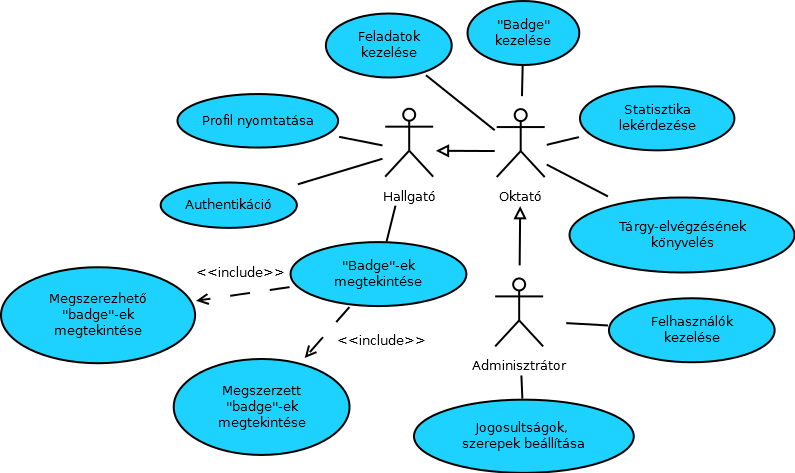
\includegraphics[width=1.00\textwidth]{figures/use_case.png}
\caption{A rendszer leírásából készített use case diagram \label{fig:use_case}}
\end{figure}

\subsection{A hallgató által elérhető funkciók}

A hallgató képes a rendszerbe bejelentkezni, profilját kinyomtatni és a ''badge''-eket megtekinteni. Ezen utolsó használati eset magába foglalja a már megszerzett és még megszerezhető ''badge''-ek megtekintését.

\subsection{Az oktató által elérhető funkciók}

Az oktató a hallgató használati eseteit is eléri (az oktató a hallgatóból származik le), kiegészítve a feladatok és ''badge''-ek kezelésével (új létrehozása, módosítása, törlése, feladat - cél - ''badge'' összerendelés elvégzése). Ezen kívül az oktató képes statisztikák lekérdezésére, és hallgatók tárgy-elvégzésének könyvelésére. 

\subsection{Az adminisztrátor által elérhető különleges funkciók}

Az adminisztrátor jogkörébe tartozik új felhasználók felvétele vagy a régiek törlése, és a felhasználók jogainak/szerepeinek (oktató vagy hallgató státusz beállítása) megadása, ezen kívül az oktatóból származik le, ezért örökli a nála felmerülő használati eseteket is.

\section{A rendszer architektúrája}

Webes alkalmazások esetében a háromrétegű architektúrát alkalmazzák. Ez, ahogy azt \aref{fig:3tier_simple}.~ábrán is mutatja, a webszerver, alkalmazásszerver és adatbázisszerver rétegeiből épül fel. Az alkalmazás szerver hivatott az adatbázisszerver által szolgáltatott adatokból előállítani azt a tartalmat, amelyet a webszerver szolgál ki a hozzá kapcsolódó klienseknek.

\begin{figure}[ht!]
\centering
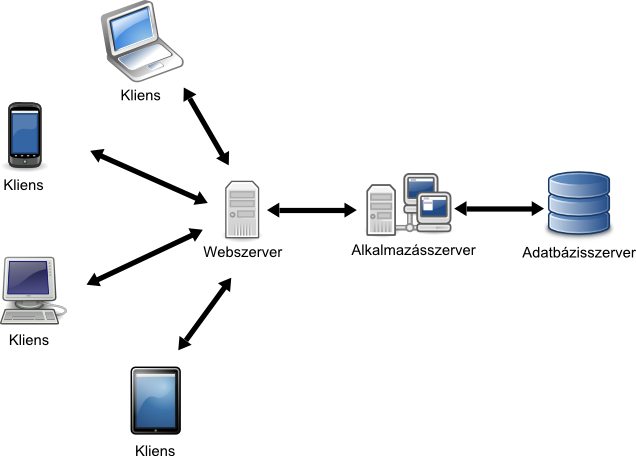
\includegraphics[width=0.50\textwidth]{figures/3tier_simple.png}
\caption{A hátom rétegű architektúra \label{fig:3tier_simple}}
\end{figure}

\section{A rendszer által használt kommunikációs protokollok}

\todo{Megírni!}

\section{A rendszer technológiai specifikációja}

\todo{Megírni!}

\section{A rendszer felhasználói felületének néhány terve}

\todo{Megírni!}

\end{document}